\documentclass[aspectratio=169, 11pt, t, xcolor={table}]{beamer}
% Slides of the English course "Computer Architecture" (same theme as the
% ENSB decks: light background, teal + orange). Compile from en/slides/.
\usepackage{amsmath, amssymb}
\usepackage{booktabs, colortbl, tabularx, array}
\usepackage{tikz}
\usepackage[skins]{tcolorbox}
\usepackage{fontawesome5}
\usepackage{listings}
\usepackage{fontspec}
\usetikzlibrary{positioning, calc, arrows.meta, shapes.geometric, decorations.pathreplacing}

\setsansfont{texgyreheros}[Extension=.otf, UprightFont=*-regular, BoldFont=*-bold,
    ItalicFont=*-italic, BoldItalicFont=*-bolditalic]
\newfontfamily\codefont[Scale=0.95, BoldFont=lmmonolt10-bold.otf,
    ItalicFont=lmmono10-italic.otf]{lmmono10-regular.otf}

\definecolor{brandTeal}{HTML}{5CC8E6}
\definecolor{brandOrange}{HTML}{FFA27F}
\definecolor{brandLight}{HTML}{F8F9FA}
\definecolor{brandDark}{HTML}{263238}
\definecolor{brandMuted}{HTML}{6C757D}
\definecolor{brandGreen}{HTML}{7BC47F}
\definecolor{brandPurple}{HTML}{B39DDB}
\colorlet{tealDeep}{brandTeal!60!black}
\colorlet{orangeDeep}{brandOrange!70!black}
\definecolor{codeGrey}{HTML}{F1F3F5}

\setbeamercolor{background canvas}{bg=brandLight}
\setbeamercolor{normal text}{fg=brandDark}
\setbeamercolor{structure}{fg=brandTeal}
\setbeamertemplate{navigation symbols}{}
\setbeamertemplate{frametitle}{%
    \vspace{0.35cm}
    \noindent{\bfseries\Large\color{brandDark}\insertframetitle}\par
    \vskip-2pt\noindent{\color{brandTeal}\rule{\textwidth}{1.5pt}}\vspace{0.05cm}}
\setbeamertemplate{footline}{%
    \hbox to \paperwidth{\hspace{0.6cm}{\color{brandMuted}\scriptsize\insertshorttitle}\hfill
        {\color{brandMuted}\scriptsize\insertframenumber\,/\,\inserttotalframenumber}\hspace{0.6cm}}%
    \vspace{0.25cm}}
\setbeamertemplate{itemize item}{\color{brandTeal}\small\faChevronRight}
\setbeamertemplate{itemize subitem}{\color{brandMuted}\small\faAngleRight}
\setbeamertemplate{enumerate item}{\color{tealDeep}\bfseries\insertenumlabel.}
% list lines are 1.4 cm apart (baseline to baseline)
\newlength{\lineGap}\setlength{\lineGap}{1.4cm}
\let\origlist\list
\def\list#1#2{\origlist{#1}{#2\setlength{\itemsep}{\dimexpr\lineGap-\baselineskip\relax}\setlength{\parsep}{0pt}}}

\newcolumntype{L}{>{\raggedright\arraybackslash}X}
\newcolumntype{C}{>{\centering\arraybackslash}X}
\newcommand{\ras}[1]{\cellcolor{brandTeal!20}\textbf{#1}}
\newcommand{\cell}[2]{\leavevmode\textcolor{#1}{#2}}
\renewcommand{\arraystretch}{1.3}
\setlength{\arrayrulewidth}{0.6pt}
\arrayrulecolor{brandMuted!70}

\tcbset{brandbox/.style={enhanced, arc=4pt, outer arc=4pt, boxrule=1.5pt,
    coltitle=white, coltext=brandDark, fonttitle=\bfseries,
    toptitle=0.8mm, bottomtitle=0.8mm, top=1.2mm, bottom=1.2mm, left=3mm, right=3mm,
    before skip=4pt, after skip=4pt}}
\newtcolorbox{tbox}[2][]{brandbox, colback=brandTeal!10, colframe=brandTeal, title={#2}, #1}
\newtcolorbox{obox}[2][]{brandbox, colback=brandOrange!10, colframe=brandOrange, title={#2}, #1}
\newtcolorbox{gbox}[2][]{brandbox, colback=brandGreen!8, colframe=brandGreen, title={#2}, #1}
\newtcolorbox{pbox}[2][]{brandbox, colback=brandPurple!10, colframe=brandPurple, title={#2}, #1}

\newcommand{\code}[1]{\mbox{\codefont\color{tealDeep}#1}}
\newcommand{\hex}[1]{\mbox{#1\textsubscript{H}}}
\newcommand{\bin}[1]{\mbox{#1\textsubscript{2}}}
\newcommand{\nql}[2]{\mbox{#1\,$\leftarrow$\,#2}}

% ---- code from ../../code/ (the verified programs of the course) ----
\lstdefinelanguage{asm86}{
    morekeywords={mov, add, adc, sub, sbb, inc, dec, neg, mul, imul, div, idiv,
        cmp, and, or, xor, not, test, shl, shr, sal, sar, rol, ror, jmp, je, jne,
        jz, jnz, jg, jge, jl, jle, ja, jae, jb, jbe, jcxz, loop, call, ret, iret,
        int, push, pop, lea, xchg, in, out, nop, movsb, rep, cld, std, cli, sti,
        syscall, addps, vaddps},
    morekeywords=[2]{org, db, dw, dd, dq, equ, proc, endp, offset, ptr, byte,
        word, dword, qword, section, global, dup, resb, rel},
    sensitive=false, morecomment=[l]{;}, morestring=[b]', morestring=[b]"}
\lstdefinestyle{base}{basicstyle=\codefont\fontsize{8}{8.6}\selectfont, columns=fullflexible,
    keepspaces=true, showstringspaces=false, upquote=true,
    keywordstyle=\color{tealDeep}\bfseries, keywordstyle=[2]\color{brandPurple!60!black}\bfseries,
    commentstyle=\color{red!75!black}, stringstyle=\color{orangeDeep},
    numbers=left, numberstyle=\tiny\color{brandMuted}, numbersep=7pt,
    firstnumber=auto,  % excerpts keep the real line numbers of the book
    xleftmargin=16pt, aboveskip=0pt, belowskip=0pt}
\lstdefinestyle{asm}{style=base, language=asm86}
\lstdefinestyle{c}{style=base, language=C}
\newtcolorbox{codebox}{enhanced, colback=codeGrey, colframe=codeGrey, boxrule=0pt, arc=2pt,
    left=3pt, right=3pt, top=2pt, bottom=2pt, before skip=3pt, after skip=3pt,
    overlay={\fill[brandTeal!70] (frame.south west) rectangle ([xshift=2.5pt]frame.north west);}}
\newtcolorbox{outbox}{enhanced, colback=brandDark, colframe=brandDark, boxrule=0pt, arc=2pt,
    left=5pt, right=5pt, top=2pt, bottom=2pt, before skip=3pt, after skip=3pt, colupper=white}
% \asm[firstline=5, lastline=20]{ch3/procnum.asm}   \cfile{...}   \screen{ch3/hello.out}
% assembly on slides: copies in code/ with inline comments removed (same lines,
% same numbers as the book; the explanation is on the slide)
\newcommand{\asm}[2][]{\begin{codebox}\lstinputlisting[style=asm,#1]{code/#2}\end{codebox}}
% smaller code for programs with long comments
\newcommand{\codesize}{\codefont\fontsize{7}{7.5}\selectfont}
\newcommand{\asms}[2][]{\begin{codebox}\lstinputlisting[style=asm,basicstyle=\codesize,#1]{code/#2}\end{codebox}}
\newcommand{\cfiles}[2][]{\begin{codebox}\lstinputlisting[style=c,basicstyle=\codesize,#1]{../../code/#2}\end{codebox}}
\newcommand{\cfile}[2][]{\begin{codebox}\lstinputlisting[style=c,#1]{../../code/#2}\end{codebox}}
\newcommand{\screen}[2][]{\begin{outbox}\lstinputlisting[basicstyle=\codefont\fontsize{8}{8.6}\selectfont\color{white},
    columns=fullflexible, keepspaces=true, aboveskip=0pt, belowskip=0pt,#1]{../../code/#2}\end{outbox}}

\tikzset{
    sahm/.style={-{Stealth[length=2.4mm]}, thick, color=brandMuted},
    sahmT/.style={-{Stealth[length=2.4mm]}, very thick, color=tealDeep},
    sahmO/.style={-{Stealth[length=2.4mm]}, very thick, color=orangeDeep},
    unit/.style={draw=#1, fill=#1!15, very thick, rounded corners=4pt,
        align=center, font=\bfseries\small, inner sep=4pt, text=brandDark},
    unit/.default=brandTeal,
    reg/.style={draw=brandDark, fill=white, thick, minimum height=0.6cm,
        font=\codefont\small, inner sep=2pt},
    % styles with a colour argument must be defined here, not inside a frame
    layer/.style={draw=#1, fill=#1!15, very thick, minimum width=9cm, minimum height=0.7cm, font=\small},
    evo/.style={unit=#1, minimum width=2.6cm, minimum height=1.2cm, font=\small},
}

% Title slide: \cover{Chapter 1}{Title}{subtitle}
\newcommand{\cover}[3]{%
\begin{frame}[plain]
    \begin{tikzpicture}[remember picture, overlay]
        \draw[brandTeal, line width=1.5pt, opacity=0.3] (current page.south east) ++(-1,1) circle (4cm);
        \draw[brandTeal, line width=0.8pt, opacity=0.25] (current page.north west) ++(2,2) circle (6cm);
        \draw[brandOrange, line width=0.5pt, opacity=0.25] (current page.north west) ++(2,2) circle (7cm);
        \begin{scope}[shift={([xshift=-1.6cm, yshift=-1.4cm]current page.north east)}, scale=0.35]
            \fill[brandDark] (-1.5,-1.5) rectangle (1.5,1.5);
            \fill[brandTeal] (-1,-1) rectangle (1,1);
            \foreach \i in {-1.2,-0.6,0,0.6,1.2} {
                \draw[brandMuted, line width=1pt] (\i,1.5) -- (\i,2); \draw[brandMuted, line width=1pt] (\i,-1.5) -- (\i,-2);
                \draw[brandMuted, line width=1pt] (1.5,\i) -- (2,\i); \draw[brandMuted, line width=1pt] (-1.5,\i) -- (-2,\i);}
        \end{scope}
    \end{tikzpicture}
    \vspace{1.4cm}
    \begin{minipage}{0.85\textwidth}
        {\color{tealDeep}\bfseries Computer Architecture \textbullet\ #1}\\[0.3cm]
        {\color{brandDark}\LARGE\bfseries #2\par}\vspace{0.3cm}
        {\color{brandMuted}\large #3}
    \end{minipage}
    \vspace{1.2cm}
    \begin{minipage}{0.85\textwidth}
        \color{brandMuted}\small
        \begin{tabular}{@{}ll}
            \textbf{Teacher:} & Dr. Benabderrezak Youcef \\
            \textbf{Course:} & UEF31, Architecture des ordinateurs \\
        \end{tabular}
    \end{minipage}
\end{frame}}

\title[Ch. 2: Inside the processor]{Inside the Processor}

\begin{document}

\cover{Chapter 2}{Inside the Processor}{registers, UAL, control unit, instructions, addressing modes, instruction cycle}

\begin{frame}{Goals of this chapter}
    \begin{tbox}{\faBullseye\quad At the end, you can:}
        \begin{itemize}
            \item describe the registers, the UAL and the control unit;
            \item compute flags and add binary numbers like an adder circuit;
            \item name the addressing modes and follow the instruction cycle.
        \end{itemize}
    \end{tbox}
\end{frame}

\begin{frame}{A look inside the processor}
    \begin{center}
    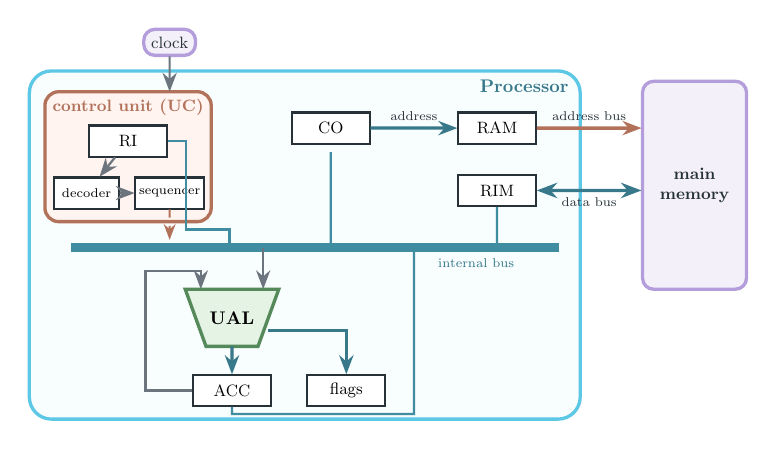
\begin{tikzpicture}[scale=0.66, transform shape, r/.style={reg, minimum width=1.5cm},
        bus/.style={line width=3pt, color=brandTeal!70!black},
        link/.style={thick, color=brandTeal!70!black},
        sig/.style={dashed, thick, color=orangeDeep, -{Stealth[length=2mm]}}]
        \draw[brandTeal, very thick, rounded corners=8pt, fill=brandTeal!4] (-8.4,-3.3) rectangle (2.2,3.4);
        \node[font=\bfseries, text=tealDeep, anchor=north east] at (2.1,3.35) {Processor};
        \draw[bus] (-7.6,0) -- (1.8,0);
        \node[font=\scriptsize, text=tealDeep] at (0.2,-0.3) {internal bus};
        \draw[orangeDeep, very thick, rounded corners=5pt, fill=brandOrange!12] (-8.1,0.5) rectangle (-4.9,3.0);
        \node[font=\small\bfseries, text=orangeDeep] at (-6.5,2.7) {control unit (UC)};
        \node[r] (ri) at (-6.5,2.05) {RI};
        \node[reg, font=\scriptsize, minimum width=1.25cm] (dec) at (-7.3,1.05) {decoder};
        \node[reg, font=\scriptsize, minimum width=1.25cm] (seq) at (-5.7,1.05) {sequencer};
        \draw[sahm] (ri) -- (dec); \draw[sahm] (dec) -- (seq);
        \draw[link] (ri.east) -- ++(0.35,0) |- (-4.55,0.35) -- (-4.55,0);
        \node[unit=brandPurple, font=\small] (clk) at (-5.7,3.95) {clock};
        \draw[sahm] (clk) -- (-5.7,3.0);
        \node[r] (co) at (-2.6,2.3) {CO};
        \node[r] (ram) at (0.6,2.3) {RAM};
        \node[r] (rim) at (0.6,1.1) {RIM};
        \draw[sahmT] (co) -- node[above, font=\scriptsize, text=brandDark] {address} (ram);
        \draw[link] (co.south) ++(0,-0.15) -- (-2.6,0);
        \draw[link] (rim.south) -- (0.6,0);
        \draw[brandGreen!70!black, very thick, fill=brandGreen!20] (-5.4,-0.8) -- (-3.6,-0.8) -- (-4.0,-1.9) -- (-5.0,-1.9) -- cycle;
        \node[font=\bfseries] at (-4.5,-1.35) {UAL};
        \node[r] (acc) at (-4.5,-2.75) {ACC};
        \node[r, font=\small] (fl) at (-2.3,-2.75) {flags};
        \draw[sahmT] (-4.5,-1.9) -- (acc.north);
        \draw[sahmT] (-3.8,-1.6) -| (fl.north);
        \draw[sahm] (-3.9,0) -- (-3.9,-0.8);
        \draw[sahm] (acc.west) -- ++(-0.9,0) |- (-6.0,-0.45) -| (-5.1,-0.8);
        \draw[link] (acc.south) -- (-4.5,-3.2) -- (-1.0,-3.2) -- (-1.0,0);
        \draw[sig] (seq.south) -- (-5.7,0.15);
        \node[unit=brandPurple, minimum width=2cm, minimum height=4cm] (mem) at (4.4,1.2) {main\\memory};
        \draw[sahmO] (ram.east) -- node[above, font=\scriptsize, text=brandDark] {address bus} ([yshift=1.1cm]mem.west);
        \draw[sahmT, {Stealth[length=2.6mm]}-{Stealth[length=2.6mm]}] (rim.east) -- node[below, font=\scriptsize, text=brandDark] {data bus} ([yshift=-0.1cm]mem.west);
    \end{tikzpicture}
    \end{center}
\end{frame}

\begin{frame}{The special registers}
    \begin{center}
    \small
    \begin{tabular}{|l|l|}
        \hline
        \ras{Register} & \ras{Keeps\dots} \\ \hline
        CO (program counter, PC / IP) & the address of the \textbf{next} instruction \\ \hline
        RI (instruction register) & the \textbf{current} instruction \\ \hline
        RAM (memory address register, MAR) & the address sent to memory \\ \hline
        RIM (memory data register, MDR) & the data coming from or going to memory \\ \hline
        ACC (accumulator) & the result of the calculation \\ \hline
    \end{tabular}
    \end{center}
    \begin{obox}{\faExclamationTriangle\quad Watch out}
        RAM the \textbf{register} (French books) is not RAM the \textbf{memory}.
    \end{obox}
\end{frame}

\begin{frame}{Why registers? Speed}
    \begin{center}
    \begin{tabular}{|c|c|c|}
        \hline
        \ras{Place} & \ras{Access time} & \ras{If a cycle were one second\dots} \\ \hline
        register & < 1 ns & one second \\ \hline
        RAM & about 80 ns & a minute and a half \\ \hline
        SSD & about 100 µs & more than a day \\ \hline
    \end{tabular}
    \end{center}
    \begin{pbox}{\faSmile\quad Analogy}
        Registers are the scrap paper on your desk; memory is the library.
    \end{pbox}
\end{frame}

\begin{frame}{The flags}
    \begin{center}
    \begin{tabular}{|c|l|l|}
        \hline
        \ras{Flag} & \ras{Becomes 1 when\dots} & \ras{Example (8 bits)} \\ \hline
        ZF & the result is zero & $5 - 5$ \\ \hline
        CF & a carry leaves the last bit & $200 + 100 > 255$ \\ \hline
        SF & the result is negative & $3 - 7$ \\ \hline
        OF & the signed result is wrong & $100 + 50 > 127$ \\ \hline
    \end{tabular}
    \end{center}
    Flags are used later to \textbf{decide}: ``if the result is zero, jump''.
\end{frame}

\begin{frame}{CF or OF? One byte, two readings}
    \begin{itemize}
        \item unsigned: 0 to 255 \qquad signed: $-128$ to $+127$ (bit 7 = sign)
    \end{itemize}
    \begin{gbox}{\faShoePrints\quad $100 + 50$}
        $\bin{0110\,0100} + \bin{0011\,0010} = \bin{1001\,0110} = 150$: no carry, so CF = 0.\\
        But bit 7 = 1: signed it reads $-106$. Two positives gave a negative, so OF = 1.
    \end{gbox}
\end{frame}

\begin{frame}{The half adder}
    \begin{columns}
        \column{0.4\textwidth}
        \begin{center}
        \begin{tabular}{|c|c||c|c|}
            \hline \ras{$A$} & \ras{$B$} & \ras{$S$} & \ras{$C$} \\ \hline
            0&0&0&0 \\ \hline 0&1&1&0 \\ \hline 1&0&1&0 \\ \hline 1&1&0&\cell{orangeDeep}{1} \\ \hline
        \end{tabular}
        \end{center}
        \column{0.55\textwidth}
        \begin{center}
        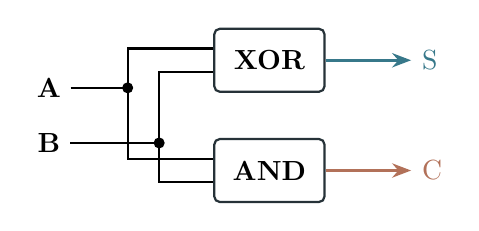
\begin{tikzpicture}[gate/.style={draw=brandDark, fill=white, thick, minimum width=1.4cm,
                minimum height=0.8cm, font=\codefont\bfseries, rounded corners=2pt}]
            \node[gate] (x) at (0,0.7) {XOR}; \node[gate] (a) at (0,-0.7) {AND};
            \node[font=\bfseries] (A) at (-2.8,0.35) {A}; \node[font=\bfseries] (B) at (-2.8,-0.35) {B};
            \fill (-1.8,0.35) circle (2pt); \fill (-1.4,-0.35) circle (2pt);
            \draw[thick] (A) -- (-1.8,0.35) |- ([yshift=0.15cm]x.west); \draw[thick] (-1.8,0.35) |- ([yshift=0.15cm]a.west);
            \draw[thick] (B) -- (-1.4,-0.35) |- ([yshift=-0.15cm]x.west); \draw[thick] (-1.4,-0.35) |- ([yshift=-0.15cm]a.west);
            \draw[sahmT] (x.east) -- (1.8,0.7) node[right] {S}; \draw[sahmO] (a.east) -- (1.8,-0.7) node[right] {C};
        \end{tikzpicture}
        \end{center}
    \end{columns}
    \begin{tbox}{\faLightbulb\quad Half adder}
        $S = A \oplus B$ \qquad $C = A \cdot B$
    \end{tbox}
\end{frame}

\begin{frame}{The 4-bit adder}
    \begin{center}
    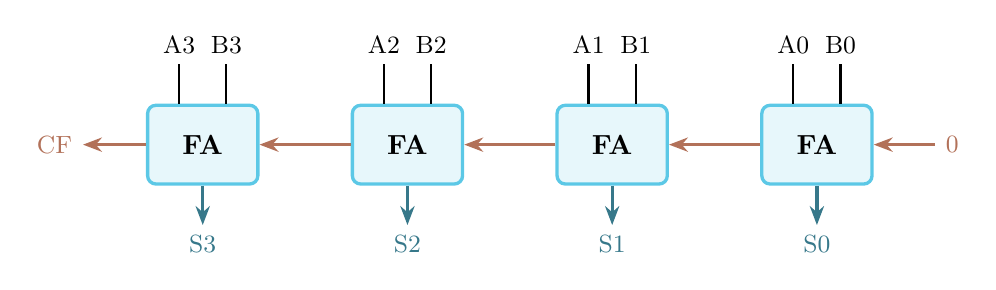
\begin{tikzpicture}[fa/.style={draw=brandTeal, fill=brandTeal!15, very thick, minimum width=1.4cm,
            minimum height=1cm, font=\codefont\bfseries, rounded corners=3pt}]
        \foreach \i/\x in {0/0, 1/-2.6, 2/-5.2, 3/-7.8} {
            \node[fa] (f\i) at (\x,0) {FA};
            \draw[thick] ([xshift=-0.3cm]f\i.north) -- ++(0,0.5) node[above, font=\small] {A\i};
            \draw[thick] ([xshift=0.3cm]f\i.north) -- ++(0,0.5) node[above, font=\small] {B\i};
            \draw[sahmT] (f\i.south) -- ++(0,-0.5) node[below, font=\small] {S\i};
        }
        \draw[sahmO] (1.5,0) node[right, font=\small] {0} -- (f0.east);
        \draw[sahmO] (f0.west) -- (f1.east); \draw[sahmO] (f1.west) -- (f2.east); \draw[sahmO] (f2.west) -- (f3.east);
        \draw[sahmO] (f3.west) -- ++(-0.8,0) node[left, font=\small] {CF};
    \end{tikzpicture}
    \end{center}
    Full adder: $S = A \oplus B \oplus C_{in}$. The carry moves from bit 0 to bit 3, like on paper.
\end{frame}

\begin{frame}{Subtracting with the same adder}
    \begin{gbox}{\faShoePrints\quad $7 - 5 = 7 + (-5)$ on 4 bits}
        \begin{enumerate}
            \item $-5$: flip $0101 \rightarrow 1010$, add 1 $\rightarrow 1011$ (two's complement).
            \item $0111 + 1011 = 1\,0010$; drop the carry: $0010 = 2$.
        \end{enumerate}
    \end{gbox}
    To \textbf{compare}: compute $A - B$, keep only the flags (ZF, CF).
\end{frame}

\begin{frame}{A real test: the flags on the 8086}
    \asm{ch2/flags.asm}
    We ran this program in the emulator. Next slide: the flags after each line.
\end{frame}

\begin{frame}{The flags after each line (real run)}
    \renewcommand{\arraystretch}{1.12}
    \begin{center}
    \begin{tabular}{|c|l|c|c|c|c|c|}
        \hline \ras{Line} & \ras{Instruction} & \ras{AL} & \ras{CF} & \ras{ZF} & \ras{SF} & \ras{OF} \\ \hline
        4 & \code{add al, 100} ($200 + 100$) & 44 & \cell{orangeDeep}{1} & 0 & 0 & 0 \\ \hline
        5 & \code{mov al, 100} & 100 & 1 & 0 & 0 & 0 \\ \hline
        6 & \code{add al, 50} ($100 + 50$) & 150 & 0 & 0 & 1 & \cell{orangeDeep}{1} \\ \hline
        8 & \code{sub al, 5} ($5 - 5$) & 0 & 0 & \cell{orangeDeep}{1} & 0 & 0 \\ \hline
        10 & \code{sub al, 7} ($3 - 7$) & 252 & \cell{orangeDeep}{1} & 0 & \cell{orangeDeep}{1} & 0 \\ \hline
    \end{tabular}
    \end{center}
    \begin{itemize}
        \item $300 - 256 = 44$: the extra 256 goes into CF.
        \item Line 5: \code{mov} does not change the flags, so CF stays 1.
    \end{itemize}
\end{frame}

\begin{frame}{The control unit}
    \begin{tbox}{\faLightbulb\quad Definition}
        The control unit reads and decodes each instruction, then sends \textbf{signals} to the other parts at each clock pulse.
    \end{tbox}
    \begin{center}
    \small
    \begin{tabular}{|c|l|}
        \hline \ras{Pulse} & \ras{Micro-operation (fetch)} \\ \hline
        T1 & \nql{RAM}{CO} \\ \hline
        T2 & \nql{RIM}{[RAM]}, \nql{CO}{CO + 1} \\ \hline
        T3 & \nql{RI}{RIM} \\ \hline
    \end{tabular}
    \end{center}
\end{frame}

\begin{frame}{Hardwired or microprogrammed?}
    \begin{center}
    \begin{tabularx}{0.95\linewidth}{|>{\centering\arraybackslash}p{2.4cm}|L|L|}
        \hline
        \ras{} & \ras{Hardwired} & \ras{Microprogrammed} \\ \hline
        Idea & fixed logic circuit & a small program per instruction \\ \hline
        Speed & very fast & a little slower \\ \hline
        Changes & hard & easy \\ \hline
        Found in & RISC & CISC (8086) \\ \hline
    \end{tabularx}
    \end{center}
    \begin{pbox}{\faSmile\quad Analogy}
        A conductor: plays nothing, but says who plays when.
    \end{pbox}
\end{frame}

\begin{frame}{The shape of an instruction}
    \begin{center}
    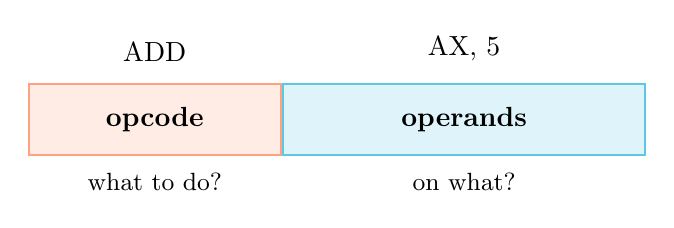
\begin{tikzpicture}
        \node[draw=brandOrange, fill=brandOrange!20, thick, minimum width=3.2cm, minimum height=0.9cm, font=\bfseries] (op) at (0,0) {opcode};
        \node[draw=brandTeal, fill=brandTeal!20, thick, minimum width=4.6cm, minimum height=0.9cm, font=\bfseries, anchor=west] (oper) at (op.east) {operands};
        \node[below=0.1cm of op, font=\small] {what to do?};
        \node[below=0.1cm of oper, font=\small] {on what?};
        \node[above=0.15cm of op, font=\codefont] {ADD};
        \node[above=0.15cm of oper, font=\codefont] {AX, 5};
    \end{tikzpicture}
    \end{center}
    \begin{itemize}
        \item \textbf{Assembly}: \code{add al, 5} \quad machine code: \texttt{04 05}.
        \item A $k$-bit opcode gives at most $2^k$ instructions ($2^8 = 256$).
    \end{itemize}
\end{frame}

\begin{frame}{Number of addresses: $A = B + C$}
    \begin{center}
    \begin{tabular}{|l|l|c|}
        \hline \ras{Machine} & \ras{Program} & \ras{Instructions} \\ \hline
        3 addresses & \code{ADD A, B, C} & 1 \\ \hline
        2 addresses (8086) & \code{MOV A, B} / \code{ADD A, C} & 2 \\ \hline
        1 address (accumulator) & \code{LOAD B} / \code{ADD C} / \code{STORE A} & 3 \\ \hline
        0 address (stack) & \code{PUSH B} / \code{PUSH C} / \code{ADD} / \code{POP A} & 4 \\ \hline
    \end{tabular}
    \end{center}
    Shorter instructions, but more of them.
\end{frame}

\begin{frame}{Classes of instructions, CISC and RISC}
    \begin{center}
    \begin{tabular}{|l|l|}
        \hline \ras{Class} & \ras{Examples} \\ \hline
        transfer & \code{MOV}, \code{PUSH}, \code{POP} \\ \hline
        arithmetic & \code{ADD}, \code{SUB}, \code{MUL} \\ \hline
        logic & \code{AND}, \code{OR}, \code{XOR}, \code{SHL} \\ \hline
        flow control & \code{JMP}, \code{JE}, \code{CALL}, \code{RET} \\ \hline
        input/output & \code{IN}, \code{OUT}, \code{INT} \\ \hline
    \end{tabular}
    \end{center}
    \textbf{CISC}: many complex instructions (x86). \textbf{RISC}: few simple ones (ARM, RISC-V).
\end{frame}

\begin{frame}{Addressing modes}
    \renewcommand{\arraystretch}{1.12}
    \begin{center}
    \small
    \begin{tabular}{|l|l|l|}
        \hline \ras{Mode} & \ras{Example} & \ras{Where is the data?} \\ \hline
        immediate & \code{mov ax, 5} & in the instruction \\ \hline
        register & \code{mov bx, ax} & in a register \\ \hline
        direct & \code{mov cx, [val]} & memory, address in the instruction \\ \hline
        indirect & \code{mov dx, [si]} & memory, address in a register \\ \hline
        indexed & \code{mov ax, [tab+di]} & start address + index \\ \hline
        relative & \code{jmp next} & current address + offset \\ \hline
    \end{tabular}
    \end{center}
    \begin{pbox}{\faSmile\quad Analogy}
        Give the book, give the shelf number, or give a paper with the shelf number.
    \end{pbox}
\end{frame}

\begin{frame}{The modes in a real program}
    \asm{ch2/modes.asm}
    \small Results (real run): AX = 0005, BX = 0005, CX = 1234, SI = 0117 (an address), DX = 1234, then AX = 001E = 30.
    \code{[ ]} always means the \textbf{content} of memory.
\end{frame}

\begin{frame}{The instruction cycle}
    \begin{columns}
        \column{0.5\textwidth}
        \begin{center}
        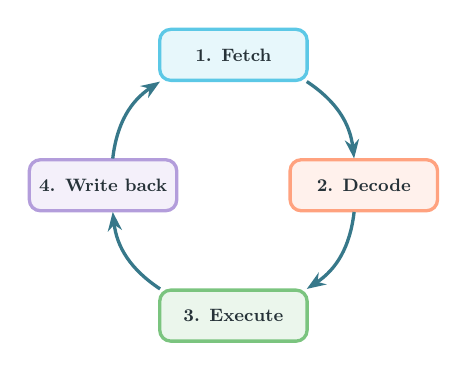
\begin{tikzpicture}[scale=0.72, transform shape]
            \foreach \a/\t/\c in {90/{1. Fetch}/brandTeal, 0/{2. Decode}/brandOrange,
                                  -90/{3. Execute}/brandGreen, 180/{4. Write back}/brandPurple}
                \node[unit=\c, minimum width=2.6cm, minimum height=0.9cm] (n\a) at (\a:2.3) {\t};
            \draw[sahmT] (n90) to[bend left=25] (n0); \draw[sahmT] (n0) to[bend left=25] (n-90);
            \draw[sahmT] (n-90) to[bend left=25] (n180); \draw[sahmT] (n180) to[bend left=25] (n90);
        \end{tikzpicture}
        \end{center}
        \column{0.47\textwidth}
        \small
        \begin{enumerate}
            \item read the instruction, CO + 1
            \item understand the opcode
            \item compute in the UAL
            \item store the result, update flags
        \end{enumerate}
    \end{columns}
\end{frame}

\begin{frame}{Step by step: \code{ADD 21} (ACC = 7, [21] = 5)}
    \begin{center}
    \small
    \begin{tabular}{|c|l|c|c|c|c|}
        \hline
        \ras{Step} & \ras{What happens} & \ras{CO} & \ras{RAM} & \ras{RIM} & \ras{ACC} \\ \hline
        fetch & \nql{RAM}{CO}, \nql{RIM}{[11]}, \nql{RI}{RIM}, CO + 1 & \cell{orangeDeep}{12} & 11 & \code{ADD 21} & 7 \\ \hline
        decode & ``add the content of address 21'' & 12 & 11 & \code{ADD 21} & 7 \\ \hline
        execute & \nql{RAM}{21}, \nql{RIM}{[21]}, UAL: $7 + 5$ & 12 & \cell{orangeDeep}{21} & \cell{orangeDeep}{5} & 7 \\ \hline
        write back & \nql{ACC}{12}, update the flags & 12 & 21 & 5 & \cell{orangeDeep}{\textbf{12}} \\ \hline
    \end{tabular}
    \end{center}
    The next instruction, \code{STORE 22}, writes 12 in memory: $z = x + y = 12$.
\end{frame}

\begin{frame}{Practice}
    \begin{obox}{\faEdit\quad Try it}
        \begin{enumerate}
            \item $1011 + 0110$ on 4 bits: result and CF? \hfill \textcolor{brandMuted}{0001, CF = 1}
            \item $10 - 20$ on 8 bits: AL and CF? \hfill \textcolor{brandMuted}{\hex{F6}, CF = 1}
            \item Mode of \code{mov al, [bx]}? \hfill \textcolor{brandMuted}{register indirect}
        \end{enumerate}
    \end{obox}
\end{frame}

\begin{frame}{Summary}
    \begin{tbox}{\faCheckCircle\quad Remember}
        \begin{itemize}
            \item Registers are tiny and fast; flags describe the last result.
            \item The UAL adds with gates, and subtracts with the two's complement.
            \item Every instruction: fetch, decode, execute, write back.
        \end{itemize}
    \end{tbox}
\end{frame}

\end{document}
